\documentclass[paper=a4, fontsize=9pt]{scrartcl}
\usepackage[bottom=0.9in, left=0.7in, right=0.7in, top=0.8in, foot=0.5in]{geometry}
\usepackage{layouts}

\usepackage[usenames,dvipsnames,x11names]{xcolor}

\usepackage[T1]{fontenc}
\usepackage{fourier}
\usepackage[english]{babel}
\usepackage{amsmath,amsfonts,amsthm}

\usepackage{sectsty}
\allsectionsfont{\centering \normalfont\scshape}

\usepackage{acronym}
\usepackage{booktabs}
\usepackage{caption}
\usepackage{fancyhdr}
\usepackage{float}
\usepackage{graphicx}
\usepackage[htt]{hyphenat}
\usepackage{lastpage}
\usepackage{multicol}
\usepackage{titlesec}
\usepackage[inline]{enumitem}
\usepackage{algorithm, algpseudocode}

\usepackage{tikz} % To generate the plot from csv
\usepackage{pgfplots, pgfplotstable}
\pgfplotsset{compat=1.5}
\usepgfplotslibrary{colorbrewer}

\pagestyle{fancyplain}
\fancyhead{}
\fancyfoot[L]{}
\fancyfoot[C]{\thepage~of~4}
\renewcommand{\headrulewidth}{0pt}
\renewcommand{\footrulewidth}{0pt}
\setlength{\headheight}{13.6pt}

\newcommand{\horrule}[1]{\rule{\linewidth}{#1}}

\title{
\vspace{-1cm}
\normalfont \normalsize
\textsc{Norwegian University of Science and Technology\\IT3708 -- Bio-Inspired Artificial Intelligence}
\horrule{0.5pt} \\[0cm]
\Huge Project 3: Segmentation of Color Image\\Using Multi-Objective Evaluation Algorithm\\[-0.3cm]
\horrule{2pt} \\[0.1cm]
}

\author{Per Magnus Veierland\\permve@stud.ntnu.no}

\date{\normalsize\today}

\newacro{MOEA}{Multi-Objective Evolutionary Algorithm}
\newacro{MST}{Minimum Spanning Tree}

\begin{document}

\maketitle

\setlength\columnsep{20pt}

\begin{multicols}{2}

% Describe  your  implementation,  only  for  MOEA  optimizing  three  objectives.  Your  description should  include  every  step  of  your  implementation  including  representation  and  evolutionary operators. Using figure(s) for chromosome is a must. (2p)

\section*{Image segmentation}

% How does your MOEA find segmentation? (0.5p)

The described system implemented in C++ performs the task of image segmentation through \ac{MOEA} using the NSGA-II algorithm \cite{deb2002fast} with the three objective functions; \textit{overall deviation}, \textit{edge value}, and \textit{connectivity measure}. Each individual chromosome in the population encodes a set of graphs where each separate graph describes an image segment. The encoding is capable of encoding any possible non-intersecting and non-overlapping image segmentation. Evolution shapes the individuals in the population according to the provided objective functions to find the set of graphs which describes the best segmentation of the input image.

To allow for efficient experimentation and evaluation, all benchmark images were scaled while respecting their aspect ratio such that their maximum dimension is 128~pixels.

The \textit{Boost Generic Image} library was used together with \textit{libjpeg} to handle images, and the \textit{Qt} library was used to render solution output images.

\section*{Chromosome representation}

The implementation uses a chromosome representation (see~Figure~\ref{figure:representation}) inspired by the graph-structure described in \cite{shirakawa2009evolutionary}. The genotype of an individual is a fixed-length sequence with length equal to the number of pixels in the input image. Each cell in the genotype contains one out of five possible values; \textit{left}, \textit{up}, \textit{down}, \textit{right}, or \textit{none}. This cell value describes how the graph node representing the input image pixel at the index of the cell is connected to its neighbors. Each graph node can connect to either a single of its four cardinal neighbors, or to itself. If a graph node at an edge of the image plane points in an outwards direction, it is treated as having the value \textit{none}. This means that all possible chromosome permutations are valid.

{
\vspace{0.3cm}
\centering
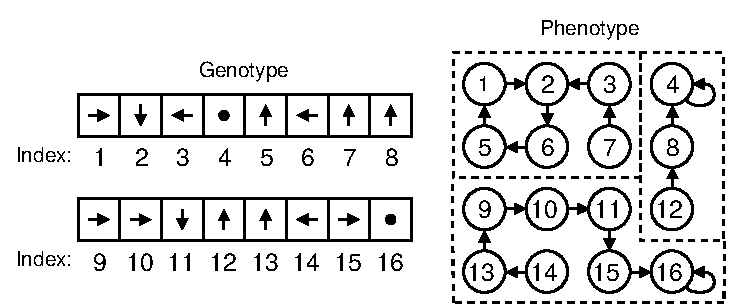
\includegraphics[scale=0.6]{figures/permve-ntnu-it3708-project-3-2017-representation.pdf}
\captionof{figure}{Image segmentation chromosome for a $4 \times 4$ pixels image. Each number represents an index in the genotype which corresponds to the pixel index in the two-dimensional input image. The dotted sections indicate the resulting image segments.}
\label{figure:representation}
\vspace{0.3cm}
}

\section*{Creation}

Initial genotype sequences are generated by constructing a \ac{MST} from the input image. This is done to provide a good starting point in the chromosome search space for image segmentation. The input image is treated as a graph where each pixel is a node connected to each of its cardinal neighbors. The weight of each edge is given by the Euclidean distance $\delta_\textsc{RGB}$ between the two neighbors in RGB color space:

\begin{equation}
\delta_\textsc{RGB} = \sqrt{\Delta R^2 + \Delta G ^2 + \Delta B ^2}
\end{equation}

From the initial image graph, \textit{Prim's algorithm} \cite{prim1957shortest} is applied from a random starting point to create a \ac{MST}. Since a random starting point is used, a different \ac{MST} is constructed as the basis of the genotype for each initial individual.

\section*{Development}

Evaluating the chromosome of an individual requires developing the genotype into a phenotype. The development process compiles the graph described by the genotype into the image segmentation description. During the development process the directions of edges in the graph described by the genotype is ignored. Starting with the first pixel node in the graph, all directly or indirectly connected pixel nodes are assigned to the same segment. This process is continued until all pixel nodes have been assigned to a segment.

\section*{Evaluation}

After compiling the image segmentation description during development, the \textit{overall deviation}, \textit{edge value}, and \textit{connectivity measure} objective functions are evaluated to produce the objective values for the individual.

\section*{Selection}

The \ac{MOEA} implementation uses a tournament selection strategy for parent selection. To select a single parent, a random sample of $k$ individuals are drawn from the population $P_t$. With a probability of $\epsilon$, a random individual is selected from the group of $k$ individuals, and with a probability of $1~-~\epsilon$; the lowest ranked individual in the group of $k$ individuals is selected according to the \textit{crowded-comparison operator} $\prec_n$ which is described in NSGA-II \cite{deb2002fast}. This procedure is performed twice to select two parents for each mating which results in two offspring.

\section*{Genetic operators}

As part of the evolution process the genetic operators crossover and mutation are used. During inheritance, a single-point crossover operation combines the genotype sequences of two parent individuals to produce two children genotype sequences.

Crossover is controlled by a crossover rate, which is a probability between $[0, 1]$ determining whether to apply the crossover operator to produce two children genotypes from two selected parent's genotypes, or to use the parent genotypes unmodified by crossover.

When applied, the mutation operator selects a random gene in a genotype sequence and sets it to a new value which is uniformly randomly selected from the set \{\textit{left}, \textit{up}, \textit{down}, \textit{right}, \textit{none}\}.

Mutation is controlled by a mutation rate, which is a probability between $[0, 1]$ determining whether to mutate an individual's genotype.

\section*{Parameters}

% Mention the values for every parameter of your chosen MOEA. (0.5p)

Table~\ref{table:parameters} lists all parameters found using trial and error which were used for all image segmentation experiments.\\[0.2cm]

{
\begin{minipage}{\linewidth{}}
\centering
\begin{tabular}{ll}
\toprule
Parameter                          & Value  \\
\midrule
Population                         & 200    \\
Generations                        & 250    \\
Crossover rate                     &   1.0  \\
Mutation rate                      &   0.05 \\
Tournament group size              &  10    \\
Tournament randomness ($\epsilon$) &   0.1  \\
\bottomrule
\end{tabular}
\captionof{table}{MOEA parameter values}
\label{table:parameters}
\end{minipage}
}

\section*{Implementation note}

To eliminate a bias introduced by the \texttt{crowding-distance-assignment} function, it was found necessary to shuffle the last front added to the next population. Otherwise, if only part of the last front is added to the next population, having the front sorted by one of the objective functions creates a significant bias towards the lower end of the last objective function sorted for. This in turn can lead to a clustering of solutions on one of the ends of the population front.

As the true Pareto front is unknown to the implementation for the problem given, $f^\text{max}_m$ and $f^\text{min}_m$ are estimated for each objective function $m$ by tracking the maximum and minimum values encountered throughout an evolutionary run for each objective.

\bibliographystyle{unsrt}
\bibliography{references.bib}

\end{multicols}

\section*{Solutions}

% For any of the test images, provide one of the segmentation examples for Pareto-optimal (for two and three objectives) solutions. You need to use the same test image for all categories (3 two objectives, 1 three objectives). You need to show both types (as Fig. 2a and 2b) of segmentation for each solution.   (1p) 

\begin{table}[H]
\centering
\begin{tabular}{ccc}
\includegraphics[width=0.3\textwidth]{{../data/deviation_edge/render_type_1_solution_3_segments_25_deviation_379206.46099_edge_203872.66667}.pdf} &
\includegraphics[width=0.3\textwidth]{{../data/deviation_edge/render_type_2_solution_3_segments_25_deviation_379206.46099_edge_203872.66667}.pdf} &
\includegraphics[width=0.3\textwidth]{{../data/deviation_edge/render_type_3_solution_3_segments_25_deviation_379206.46099_edge_203872.66667}.pdf} \\[0.15cm]
\multicolumn{3}{c}{Figure 2: Segmentation of test image \#3 using objective functions \textit{overall deviation} and \textit{edge value}.} \\
\multicolumn{3}{c}{\textit{Segment count}: 25 \quad \textit{Overall deviation}: 379206.5 \quad \textit{Edge value}: 203872.7} \\[1.8cm]

\includegraphics[width=0.3\textwidth]{{../data/edge_connectivity/render_type_1_solution_3_segments_1_edge_0.00000_connectivity_0.00000}.pdf} &
\includegraphics[width=0.3\textwidth]{{../data/edge_connectivity/render_type_2_solution_3_segments_1_edge_0.00000_connectivity_0.00000}.pdf} &
\includegraphics[width=0.3\textwidth]{{../data/edge_connectivity/render_type_3_solution_3_segments_1_edge_0.00000_connectivity_0.00000}.pdf} \\[0.15cm]
\multicolumn{3}{c}{Figure 3: Segmentation of test image \#3 using objective functions \textit{edge value} and \textit{connectivity measure}.} \\
\multicolumn{3}{c}{\textit{Segment count}: 1 \quad \textit{Edge value}: 0.0 \quad \textit{Connectivity measure}: 0.0} \\[1.8cm]

\includegraphics[width=0.3\textwidth]{{../data/deviation_connectivity/render_type_1_solution_3_segments_25_deviation_339663.80691_connectivity_2087.16667}.pdf} &
\includegraphics[width=0.3\textwidth]{{../data/deviation_connectivity/render_type_2_solution_3_segments_25_deviation_339663.80691_connectivity_2087.16667}.pdf} &
\includegraphics[width=0.3\textwidth]{{../data/deviation_connectivity/render_type_3_solution_3_segments_25_deviation_339663.80691_connectivity_2087.16667}.pdf} \\[0.15cm]
\multicolumn{3}{c}{Figure 4: Segmentation of test image \#3 using objective functions \textit{overall deviation} and \textit{connectivity measure}.} \\
\multicolumn{3}{c}{\textit{Segment count}: 25 \quad \textit{Overall deviation}: 339663.8 \quad \textit{Connectivity measure}: 2087.2} \\[1.8cm]

\includegraphics[width=0.3\textwidth]{{../data/deviation_edge_connectivity/render_type_1_solution_3_segments_25_deviation_345576.53426_edge_206196.78657_connectivity_2213.00000}.pdf} &
\includegraphics[width=0.3\textwidth]{{../data/deviation_edge_connectivity/render_type_2_solution_3_segments_25_deviation_345576.53426_edge_206196.78657_connectivity_2213.00000}.pdf} &
\includegraphics[width=0.3\textwidth]{{../data/deviation_edge_connectivity/render_type_3_solution_3_segments_25_deviation_345576.53426_edge_206196.78657_connectivity_2213.00000}.pdf} \\[0.15cm]
\multicolumn{3}{c}{Figure 5: Segmentation of test image \#3 using objective functions \textit{overall deviation}, \textit{edge value}, and \textit{connectivity measure}.} \\
\multicolumn{3}{c}{\textit{Segment count}: 25 \quad \textit{Overall deviation}: 345576.5 \quad \textit{Edge value}: 206196.8 \quad \textit{Connectivity measure}: 2213.0} \\[1.8cm]
\end{tabular}
\end{table}

\section*{Pareto fronts}

% Plot Pareto-fronts (3 two objectives, 1 three objectives) for the same solutions those you will use in Point-3.  (1p)

\pgfplotsset{
every axis/.append style={
scale only axis,
width=0.25\textwidth,height=0.25\textwidth,
},
/tikz/every picture/.append style={
trim axis left,
trim axis right,
baseline
}
}

\newcommand{\paretoscattertwodimensional}[6]{
    \pgfplotsset{cycle list/RdYlGn-9}
    \pgfplotstablesort[sort key=1,sort cmp=int >]{#1}{#2}

    \begin{tikzpicture}
    \begin{axis}[xlabel={#3},ylabel={#4},legend pos=south east,colormap name={RdYlGn-9}]
    \addplot [scatter,only marks,scatter src=explicit,scatter/use mapped color={draw opacity=0,fill=mapped color},mark size=0.8pt] table[x index=#5,y index=#6,meta index=1,col sep=space] {#1};
    \end{axis}
    \end{tikzpicture}
}

\begin{table}[H]
\centering
\begin{tabular}{cp{0.7cm}cp{0.7cm}c}
\paretoscattertwodimensional{\paretodatadeviationedge}{../data/deviation_edge/population.txt}{Overall deviation}{Edge value}{3}{4} & ~ &
\paretoscattertwodimensional{\paretodataedgeconnectivity}{../data/edge_connectivity/population.txt}{Edge value}{Connectivity measure}{3}{4} & ~ &
\paretoscattertwodimensional{\paretodatadeviationconnectivity}{../data/deviation_connectivity/population.txt}{Overall deviation}{Connectivity measure}{3}{4} \\[0.85cm]
(a) & ~ & (b) & ~ & (c) \\[0.25cm]
\multicolumn{5}{c}{\begin{minipage}{0.9\textwidth}\centering Figure 6: Plots showing the Pareto front resulting from multi-objective NSGA-2 evolution using combinations of two objective functions; \textit{overall deviation} and \textit{edge value} (a), \textit{edge value} and \textit{connectivity measure} (b), and \textit{overall deviation} and \textit{connectivity measure} (c). All final individuals belongs to the first non-dominated front.\end{minipage}} \\[1.5cm]

\multicolumn{5}{c}{
\begin{minipage}{\textwidth}
\centering
\begin{tabular}{cp{1cm}c}
{
    \pgfplotsset{cycle list/RdYlGn-9}
    \pgfplotstablesort[sort key=1,sort cmp=int >]{\paretodatadeviationedgeconnectivityx}{../data/deviation_edge_connectivity/population.txt}

    \begin{tikzpicture}
    \begin{axis}[xlabel={Overall deviation},ylabel={Edge value},zlabel={Connectivity measure},legend pos=south east,colormap name={RdYlGn-9},view/v=-20,view/az=-45,xlabel shift=-8pt]
    \addplot3[scatter,only marks,scatter/use mapped color={draw opacity=0,fill=mapped color},mark size=0.8pt] table[x index=3,y index=4,z index=5,col sep=space] {\paretodatadeviationedgeconnectivityx};
    \end{axis}
    \end{tikzpicture}
} & ~ &
{
    \pgfplotsset{cycle list/RdYlGn-9}
    \pgfplotstablesort[sort key=1,sort cmp=int >]{\paretodatadeviationedgeconnectivityy}{../data/deviation_edge_connectivity/population.txt}

    \begin{tikzpicture}
    \begin{axis}[xlabel={Overall deviation},ylabel={Edge value},zlabel={Connectivity measure},legend pos=south east,colormap name={RdYlGn-9},view/v=-20,view/az=45]
    \addplot3[scatter,only marks,scatter/use mapped color={draw opacity=0,fill=mapped color},mark size=0.8pt] table[x index=3,y index=4,z index=5,col sep=space] {\paretodatadeviationedgeconnectivityy};
    \end{axis}
    \end{tikzpicture}
} \\[1cm]
(a) & ~ & (b)\\[0.25cm]
\end{tabular}
\end{minipage}
}\\
\multicolumn{5}{c}{\begin{minipage}{0.95\textwidth}\centering Figure 7: Plots showing the Pareto front resulting from multi-objective NSGA-2 evolution using the three objective functions\\\textit{overall deviation}, \textit{edge value}, and \textit{connectivity measure}. The colors reflect the \textit{connectivity measure} and is meant to improve the readability of the plot. All final individuals belongs to the first non-dominated front.\end{minipage}} \\[1.5cm]

\paretoscattertwodimensional{\paretodatadeviationedgeconnectivitya}{../data/deviation_edge_connectivity/population.txt}{Overall deviation}{Edge value}{3}{4} & ~ &
\paretoscattertwodimensional{\paretodatadeviationedgeconnectivityb}{../data/deviation_edge_connectivity/population.txt}{Edge value}{Connectivity measure}{4}{5} & ~ &
\paretoscattertwodimensional{\paretodatadeviationedgeconnectivityc}{../data/deviation_edge_connectivity/population.txt}{Overall deviation}{Connectivity measure}{3}{5} \\[1.5cm]
\multicolumn{5}{c}{\begin{minipage}{0.95\textwidth}\centering Figure 8: Plots showing the same data as Figure~6 in three separate two-dimensional views.\end{minipage}}
\end{tabular}
\end{table}

\end{document}
